\documentclass[12pt,letterpaper, onecolumn]{exam}
\usepackage{amsmath}
\usepackage{amssymb}
\usepackage{textcomp, gensymb}
\usepackage{siunitx}
\usepackage{graphicx}
\usepackage{setspace}
\usepackage{nicefrac}
\usepackage{indentfirst}
\usepackage[lmargin=71pt, tmargin=1.2in]{geometry}

%------------------------------------------------------------
\lhead{Principles of Navigation}
\rhead{Tanner Koza}
\thispagestyle{empty}

\begin{document}

\title{Homework 2 - Principles of Navigation

    \large MECH - 6970}
\author{Tanner Koza}
\maketitle
\pointsdroppedatright
\printanswers
\renewcommand{\solution}{\noindent\textbf{Solution:}\enspace}

\begin{questions}
    \question
    Pedestrian Navigation System: Use your phone to implement a pedestrian navigation
    system. Estimate your position by starting at a known location and dead reckoning using
    an open-source step counter and compass. Make sure that your route is at least 1 km and
    contains turns in both directions. Use the compass to track your orientation. You can
    record measurements (i.e.\ step and compass reading) on your phone if you have that
    functionality. Otherwise use a pad and paper to track steps and compass changes.

    \solution
    Figure~\ref{fig:walk} depicts the GPS and dead reckoned solutions for my walk near the MRI research building on Auburn's campus. I used my watch to count steps and an average step length of $0.9 \unit{\m}$. The GPS trajectory came from a workout app on my phone that I imported into MATLAB\@. The error at the final position is $73.81 \unit{\metre}$ and the orientation error is approximately 55 degrees. The orientation error is difficult to see in the trajectory because the last two points taken were relatively close to each other. My GPS path determined I walked $1.02 \unit{\km}$ while my dead reckoned solution determined I walked $1.87 \unit{\km}$.
    \begin{figure}[!h]
        \centering
        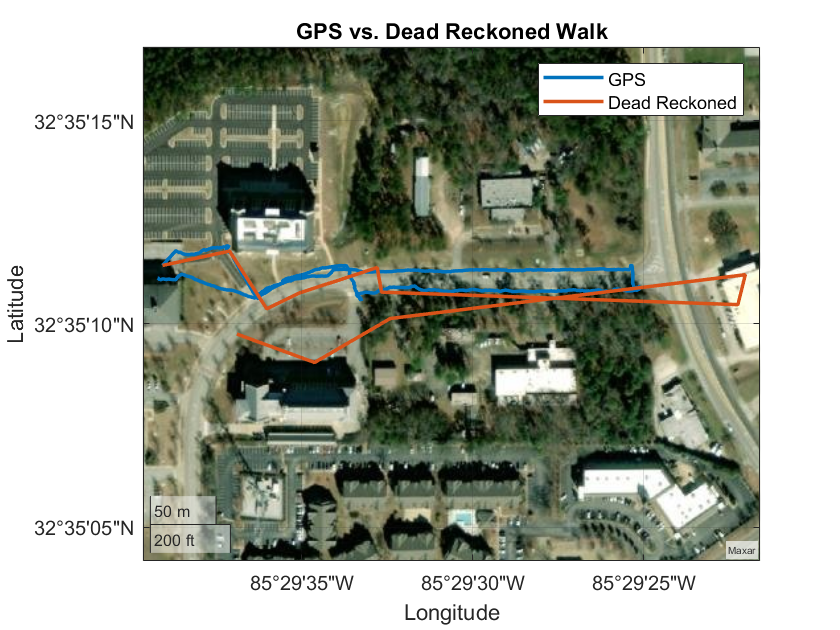
\includegraphics[width=\linewidth]{assets/HW2_P1_FIG.png}
        \caption{Dead Reckoned Walk with Compass and Constant Step Length}
        \label{fig:walk}
    \end{figure}
    \clearpage

    \question
    Find a scholarly article describing a navigation system for a team of at least two ground
    vehicles. Describe the sensors used, states estimated, and estimator architecture. Give a
    brief description of the problem statement/motivation for the work. What results were
    presented (e.g.\ plots of positioning accuracy, raw sensor data, etc.)? Did the authors
    successfully convey the methodology?

    \solution
    In "Hitchhiking Robots: A Collaborative Approach for Efficient Multi-Robot Navigation in Indoor Environments" (Ravankar et\ al.), a method of visual servoing is employed to allow a follower robot to navigate based on a leader robot's calculated solution (i.e.\ path planning, localization, etc.). This paper is motivated by the use of robot convoys in commercial warehouses. Specifically, it aims to provide a method that efficiently reduces the robots' necessary computation (and cost) by taking advantage of their repetitive nature.

    The sensors used in this paper include a Microsoft Kinect for perception, a UHG-08LX laser range sensor for inter-robot ranging, a 2D LiDAR, and wheel encoders for simultaneous localization and mapping (SLAM). The robot states include $x$ and $y$ local positions along with the heading $\theta$ of each vehicle. The hitchhiking algorithm is comprised of 4 steps: the handshake, coupling, navigation, and decoupling. The handshake step involves a hitchhiker broadcasting a request to join a leader and several heuristics being evaluated to determine whether or not two robots should couple. Once it is decided they can couple, the Kinect is used by the hitchhiker to recognize a QR code on the leader and initiate visual servoing. Once coupled, the leader begins navigating and all other localization functions performed by the hitchhiker are shut down and only visual servoing is used. Once they reach the end goal, the robots decouple and the leader passes any information accumulated in the time of visual servoing to the hitchhiker. The navigation of the leader is conducted using an Extended Kalman Filter that fuses LiDAR and wheel encoder data to provide a map and position solution.

    The results for this paper included the locations of objects transferred from the leader's frame to the hitchhiker's frame, but no path/following errors. More data about the time needed to execute each stage of the algorithm was presented. Overall, I wish they would have included more information regarding the quality of the hitchhiking, but at the end of the day, they successfully convey their approach can work.

    \clearpage

    \question
    In class we developed the basic (elementary) rotation matrix
    \begin{equation*}
        \begin{bmatrix}
            \cos(\theta) & -\sin(\theta) & 0 \\
            \sin(\theta) & \cos(\theta)  & 0 \\
            0            & 0             & 1
        \end{bmatrix}
    \end{equation*}
    that describes the orientation of a coordinate frame rotated away from another coordinate frame by an angle $\theta$ about the z-axis.

    \begin{parts}
        \part
        Derive the basic (elementary) rotation matrix $C_{y,\theta}$ that describes the orientation of a coordinate frame rotated away from another coordinate frame by an angle $\theta$ about the y-axis.

        \solution
        The rotation matrix $C_{y,\theta}$  is comprised of the same unit vector dot products that make the rotation matrix $C_{z,\theta}$. However, the $y$ and $y'$ axes are aligned in this case unlike the $z$ and $z'$ axes for $C_{z,\theta}$. This gives us the following for the frame rotation about $y$ shown in Figure~\ref{fig:yrot}.

        \begin{equation*}
            \begin{split}
                C_{y,\theta} & =
                \begin{bmatrix}
                    x'x & y'x & z'x \\
                    x'y & y'y & z'y \\
                    x'z & y'z & z'z
                \end{bmatrix} \\
                C_{y,\theta} & =
                \begin{bmatrix}
                    cos(\theta)  & 0 & sin(\theta) \\
                    0            & 1 & 0           \\
                    -sin(\theta) & 0 & cos(\theta) \\
                \end{bmatrix}
            \end{split}
        \end{equation*}

        \begin{figure}[!h]
            \centering
            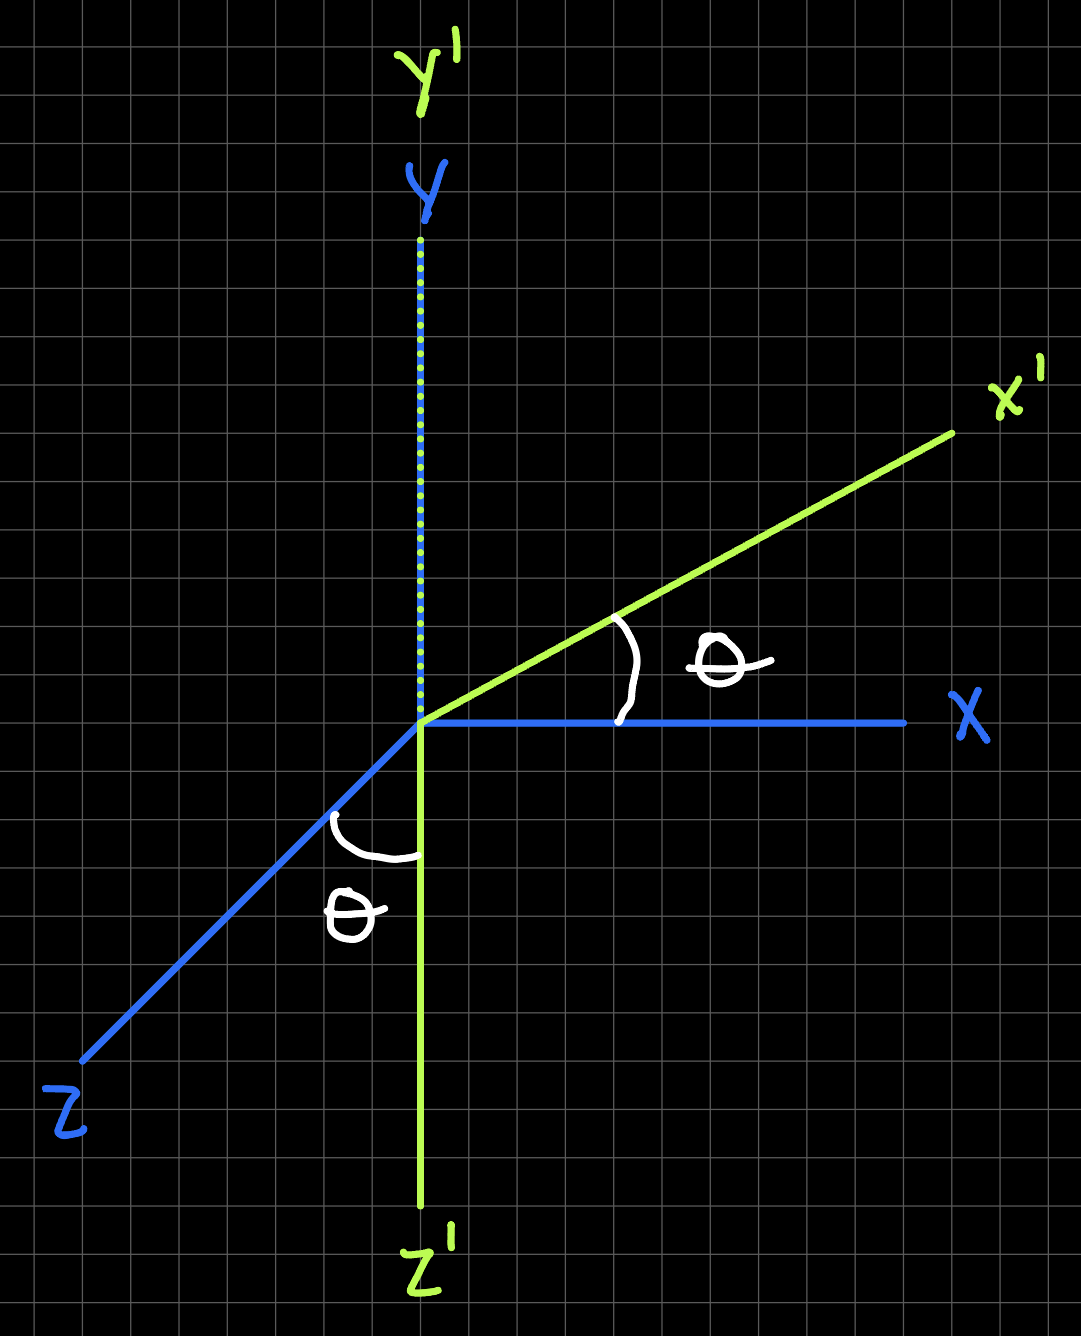
\includegraphics[scale=0.3]{assets/HW2_P3_FIG.png}
            \caption{y-axis Frame-to-Frame Rotation}
            \label{fig:yrot}
        \end{figure}

    \end{parts}

    \clearpage

    \question
    For each of the matrices below, determine which are valid rotation matrices. Justify your answer based on expected properties.

    \solution
    The validity of a rotation matrix is determined by whether or not it is orthonormal. The orthogonality can be tested by multiplying the matrix by its transpose and seeing if the result is an identity matrix. The normality can be tested by taking the determinant and seeing if the result is 1. All solutions were calculated using MATLAB.
    \begin{parts}
        \part
        \begin{equation*}
            \begin{bmatrix}
                0  & 0 & 1 \\
                0  & 1 & 0 \\
                -1 & 0 & 0
            \end{bmatrix}
        \end{equation*}

        \solution
        This matrix \textbf{IS} a valid rotation matrix. The result of the transpose multiplication is the identity and the determinant is 1.

        \begin{equation*}
            \begin{split}
                C_{b}^{a}(C_b^a)^T & =
                \begin{bmatrix}
                    1 & 0 & 0 \\
                    0 & 1 & 0 \\
                    0 & 0 & 1
                \end{bmatrix} \\
                \det{C_b^a} & = 1
            \end{split}
        \end{equation*}

        \part
        \begin{equation*}
            \begin{bmatrix}
                1 & 0 & -1 \\
                0 & 1 & 0  \\
                0 & 0 & 0
            \end{bmatrix}
        \end{equation*}

        \solution
        This matrix \textbf{IS NOT} a valid rotation matrix. The result of the transpose multiplication is not the identity and the determinant is 0.

        \begin{equation*}
            \begin{split}
                C_{b}^{a}(C_b^a)^T & =
                \begin{bmatrix}
                    2 & 0 & 0 \\
                    0 & 1 & 0 \\
                    0 & 0 & 0
                \end{bmatrix} \\
                \det{C_b^a} & = 0
            \end{split}
        \end{equation*}

        \part
        \begin{equation*}
            \begin{bmatrix}
                1 & 0           & 0 \\
                0 & \frac{1}{2} & 0 \\
                0 & 0           & 2
            \end{bmatrix}
        \end{equation*}

        \solution
        This matrix \textbf{IS NOT} a valid rotation matrix. The result of the transpose multiplication is not the identity; however, the determinant is 1.

        \begin{equation*}
            \begin{split}
                C_{b}^{a}(C_b^a)^T & =
                \begin{bmatrix}
                    1 & 0    & 0 \\
                    0 & 0.25 & 0 \\
                    0 & 0    & 4
                \end{bmatrix} \\
                \det{C_b^a} & = 1
            \end{split}
        \end{equation*}

        \part
        \begin{equation*}
            \begin{bmatrix}
                0.4330  & -0.7718 & 0.4656 \\
                0.7500  & 0.5950  & 0.2888 \\
                -0.5000 & 0.2241  & 0.8365
            \end{bmatrix}
        \end{equation*}

        \solution
        This matrix \textbf{IS} a valid rotation matrix. The result of the transpose multiplication is the identity and the determinant is 1.

        \begin{equation*}
            \begin{split}
                C_{b}^{a}(C_b^a)^T & =
                \begin{bmatrix}
                    1 & 0 & 0 \\
                    0 & 1 & 0 \\
                    0 & 0 & 1
                \end{bmatrix} \\
                \det{C_b^a} & = 1
            \end{split}
        \end{equation*}

        \part
        \begin{equation*}
            \begin{bmatrix}
                0.5000  & -0.1464 & 0.8536  \\
                0.5000  & -0.8536 & -0.1464 \\
                -0.7071 & 0.5000  & 0.5000
            \end{bmatrix}
        \end{equation*}

        \solution
        This matrix \textbf{IS NOT} a valid rotation matrix. The result of the transpose multiplication is not the identity and the determinant is -0.4572.

        \begin{equation*}
            \begin{split}
                C_{b}^{a}(C_b^a)^T & =
                \begin{bmatrix}
                    1.001 & 0.25    & 0.0001  \\
                    0.25  & 1.001   & -0.8536 \\
                    0.001 & -0.8536 & 1
                \end{bmatrix} \\
                \det{C_b^a} & = -0.4572
            \end{split}
        \end{equation*}

    \end{parts}

    \clearpage

    \question
    Consider the rotation matrix

    \begin{equation*}
        C_{0}^{1} =
        \begin{bmatrix}
            0  & \frac{-\sqrt{3}}{2} & \frac{-1}{2}       \\
            0  & \frac{-1}{2}        & \frac{\sqrt{3}}{2} \\
            -1 & 0                   & 0
        \end{bmatrix}
    \end{equation*}

    \begin{parts}

        \part
        Sketch frames 0 and 1 with their origins co-located.

        \solution
        The sketch is found in Figure~\ref{fig:colo}.

        \begin{figure}[!h]
            \centering
            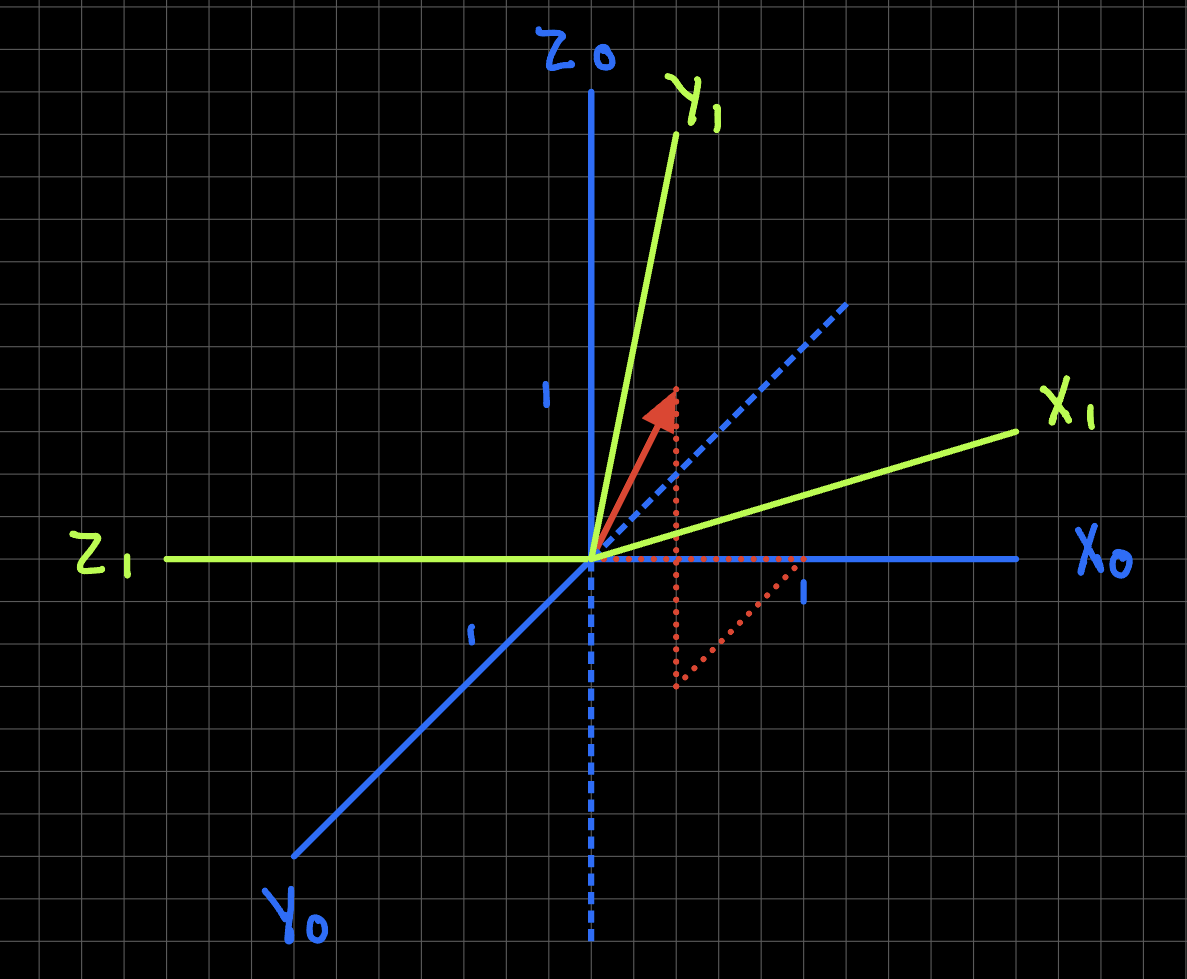
\includegraphics[scale=0.5]{assets/HW2_P5_FIG.png}
            \caption{Co-located Frame Sketch}
            \label{fig:colo}
        \end{figure}

        \part
        Given a vector $\vec{v}^{0} = [1, 1, 1]^T$ coordinatized in frame 0, re-coordinatize the vector such that it is described in frame 1.
        \solution
        \begin{equation*}
            \begin{split}
                \vec{v}^1 & = C^1_0 \vec{v}^0 \\
                \vec{v}^1 & =
                \begin{bmatrix}
                    0  & -\frac{\sqrt{3}}{2} & -\frac{1}{2}       \\
                    0  & -\frac{1}{2}        & \frac{\sqrt{3}}{2} \\
                    -1 & 0                   & 0                  \\
                \end{bmatrix}
                \begin{bmatrix}
                    1 \\
                    1 \\
                    1 \\
                \end{bmatrix}\\
                \vec{v}^1 & =
                \begin{bmatrix}
                    -1.3660 \\
                    0.3660  \\
                    -1.000  \\
                \end{bmatrix}\\
            \end{split}
            \label{}
        \end{equation*}

    \end{parts}

    \clearpage

    \question
    For each pair of coordinate frames, find the rotation matrix $C_{b}^{a}$ that describes their relative orientation.

    \begin{parts}
        \part
        \begin{figure*}[!h]
            \centering
            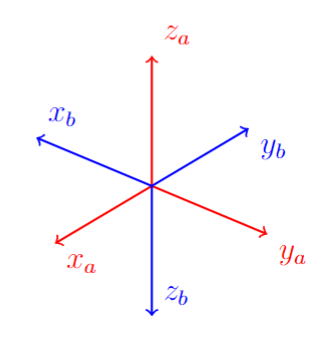
\includegraphics[scale=0.75]{assets/HW2_P6_FIG.PNG}
        \end{figure*}

        \solution
        The rotations necessary to align the above frames include a rotation of $-90 \unit{\degree}$ about the $z_b$ axis and a $180 \unit{\degree}$ rotation about the new $x_b$ axis. The rotation matrix that describes this is the following.

        \begin{equation*}
            \begin{split}
                C_b^a & = R_{z,-90}R_{x,180}\\
                C_b^a & =
                \begin{bmatrix}
                    0  & 1 & 0 \\
                    -1 & 0 & 0 \\
                    0  & 0 & 1
                \end{bmatrix}
                \begin{bmatrix}
                    1 & 0  & 0  \\
                    0 & -1 & 0  \\
                    0 & 0  & -1
                \end{bmatrix} \\
                C_b^a & =
                \begin{bmatrix}
                    0  & -1 & 0  \\
                    -1 & 0  & 0  \\
                    0  & 0  & -1
                \end{bmatrix}
            \end{split}
        \end{equation*}

        \part
        \begin{figure*}[!h]
            \centering
            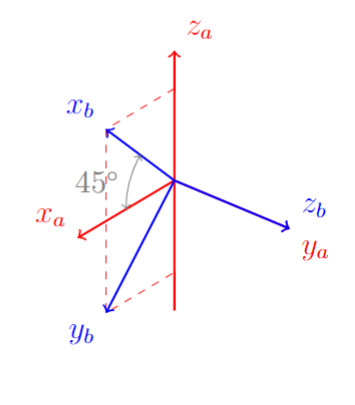
\includegraphics[scale=0.75]{assets/HW2_P6_FIG2.PNG}
        \end{figure*}

        \solution
        The rotations necessary to align the above frames include a rotation of $45 \unit{\degree}$ about the $z_b$ axis and a rotation of $90 \unit{\degree}$ about the new $x_b$ axis. The rotation matrix that describes this is the following.

        \begin{equation*}
            \begin{split}
                C_b^a & = R_{x,90}R_{z,45}\\
                C_b^a & =
                \begin{bmatrix}
                    1 & 0  & 0 \\
                    0 & 0  & 1 \\
                    0 & -1 & 0
                \end{bmatrix}
                \begin{bmatrix}
                    \frac{\sqrt{2}}{2}  & \frac{\sqrt{2}}{2} & 0 \\
                    -\frac{\sqrt{2}}{2} & \frac{\sqrt{2}}{2} & 0 \\
                    0                   & 0                  & 1
                \end{bmatrix} \\
                C_b^a & =
                \begin{bmatrix}
                    \frac{\sqrt{2}}{2} & \frac{\sqrt{2}}{2}  & 0 \\
                    0                  & 0                   & 1 \\
                    \frac{\sqrt{2}}{2} & -\frac{\sqrt{2}}{2} & 0
                \end{bmatrix}
            \end{split}
        \end{equation*}


    \end{parts}

    \clearpage

    \question
    Coordinate frame {1} is obtained from frame {0} by the following sequence of rotations:

    \begin{parts}
        \part
        $-90 \unit{\degree}$ about the fixed z-axis
        \part
        $90 \unit{\degree}$ about the current y-axis
        \part
        $-90 \unit{\degree}$ about the fixed x-axis
    \end{parts}

    Find the resulting rotation matrix $C_{1}^{0}$ and sketch frames {0} and {1} relative to each other.

    \solution
    The resulting matrix was calculated in MATLAB\@. The order of multiplication for the matrices comes from the fact that relative rotations come before fixed rotations. Figure~\ref{fig:relaxes} depicts the frames.

    \begin{equation*}
        \begin{split}
            C_1^0 & = R_xR_zR_y \\
            C_1^0 & =
            \begin{bmatrix}
                0  & 1 & 0 \\
                -1 & 0 & 0 \\
                0  & 0 & 1 \\
            \end{bmatrix}
        \end{split}
    \end{equation*}

    \begin{figure}[!h]
        \centering
        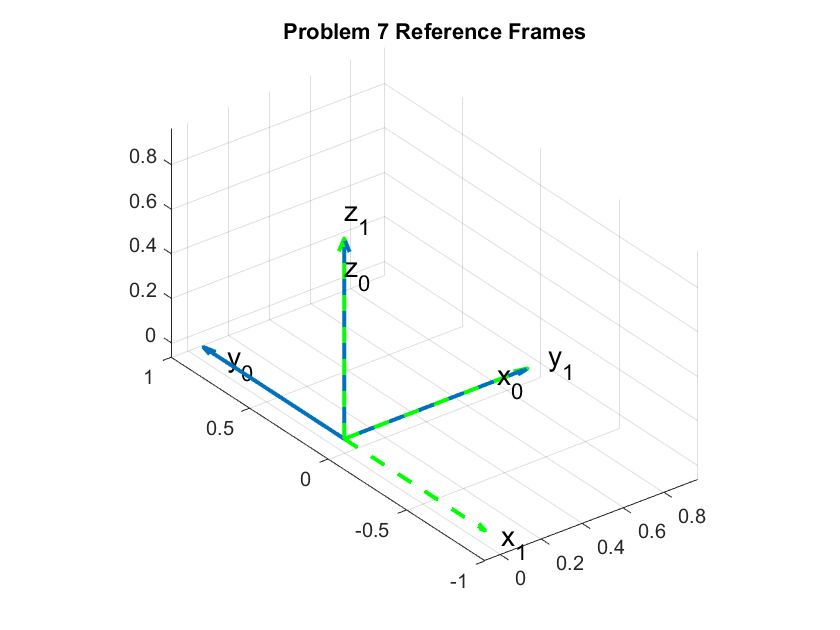
\includegraphics[width=\linewidth]{assets/HW2_P7_FIG.png}
        \caption{Relative Reference Frames}
        \label{fig:relaxes}
    \end{figure}

    \clearpage

    \question
    Given the roll-pitch-yaw angles $(\phi, \theta, \psi) = (120 \unit{\degree}, 45 \unit{\degree}, -120 \unit{\degree})$, find the rotation matrix that describes the same orientation. Assume a ZYX series of rotations. Verify that you have constructed the correct rotation matrix by backing out the angles.

    \solution
    The rotation matrix was calculated in MATLAB as so.

    \begin{equation*}
        \begin{split}
            C & = R_{\phi,120}R_{\theta,45}R_{\psi,-120} \\
            C & =
            \begin{bmatrix}
                1 & 0         & 0          \\
                0 & cos(\phi) & -sin(\phi) \\
                0 & sin(\phi) & cos(\phi)  \\
            \end{bmatrix}
            \begin{bmatrix}
                cos(\theta)  & 0 & sin(\theta) \\
                0            & 1 & 0           \\
                -sin(\theta) & 0 & cos(\theta) \\
            \end{bmatrix}
            \begin{bmatrix}
                cos(\psi) & -sin(\psi) & 0 \\
                sin(\psi) & cos(\psi)  & 0 \\
                0         & 0          & 1 \\
            \end{bmatrix} \\
            C & =
            \begin{bmatrix}
                -0.3536 & 0.6124  & 0.7071  \\
                0.1268  & 0.7803  & -0.6124 \\
                -0.9268 & -0.1268 & -0.3536 \\
            \end{bmatrix}
        \end{split}
    \end{equation*}

    The angles can be backed out using the following equations.

    \begin{equation*}
        \begin{split}
            \phi & = tan^{-1}\left(\frac{-C_{2,3}}{C_{3,3}}\right) \\
            \theta & = tan^{-1}\left(\frac{C_{1,3}}{\sqrt{C_{2,3}^2 + C_{3,3}^2}}\right) \\
            \psi & = tan^{-1}\left(\frac{-C_{1,2}}{C_{1,1}}\right) \\
        \end{split}
    \end{equation*}

    Plugging in the corresponding values results in the following Euler angles using $atan2()$ in MATLAB.

    \begin{equation*}
        \begin{split}
            \phi & = -120 \unit{\degree} \\
            \theta & = 45 \unit{\degree} \\
            \psi & = 120 \unit{\degree} \\
        \end{split}
    \end{equation*}

    \clearpage
    \question
    Consider the three coordinate frames ${\alpha}, {\beta}, {\gamma}$ shown in the diagram. Following the notation introduced in class, find the following Cartesian position vectors (denoted by $\vec{r})$ and rotation matrices (denoted by $C$).

    \begin{figure*}[!h]
        \centering
        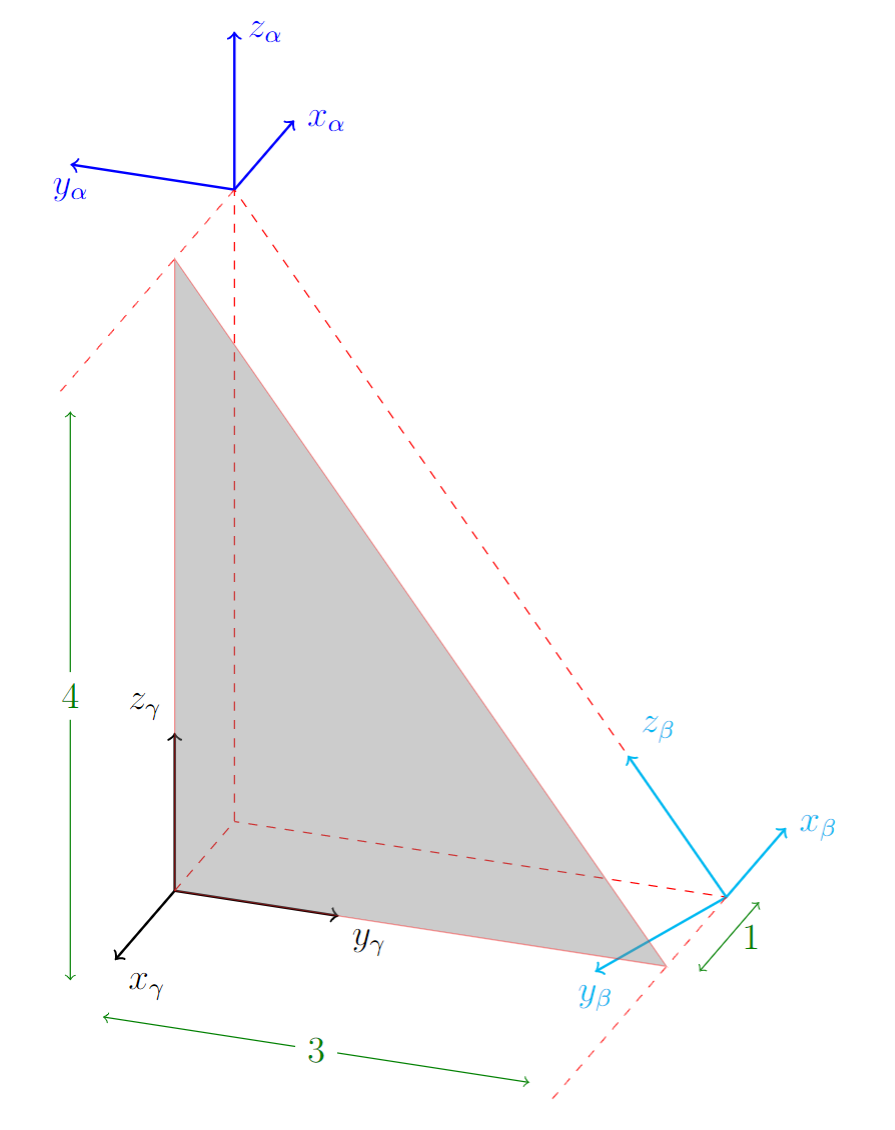
\includegraphics[scale=0.75]{assets/HW2_P9_FIG.PNG}
    \end{figure*}

    \begin{parts}
        \part
        $\vec{r}_{\gamma \alpha}^{\gamma}$

        \solution
        $\vec{r}_{\gamma \alpha}^{\gamma}$ can be found by subtracting the vector components from $\gamma$ to $\alpha$ in the $\gamma$ frame.

        \begin{equation*}
            \begin{split}
                \vec{r}_{\gamma \alpha}^{\gamma} & =
                \begin{bmatrix}
                    \alpha_x - \gamma_x \\
                    \alpha_y - \gamma_y \\
                    \alpha_z - \gamma_z \\
                \end{bmatrix} \\
                \vec{r}_{\gamma \alpha}^{\gamma} & =
                \begin{bmatrix}
                    -1 - 0 \\
                    0-0    \\
                    4 - 0  \\
                \end{bmatrix} \\
                \vec{r}_{\gamma \alpha}^{\gamma} & =
                \begin{bmatrix}
                    -1 \\
                    0  \\
                    4  \\
                \end{bmatrix} \\
            \end{split}
        \end{equation*}

        \part
        $\vec{r}_{\gamma \beta}^{\gamma}$
        \solution
        $\vec{r}_{\gamma \beta}^{\gamma}$ can be found by subtracting the vector components from $\gamma$ to $\beta$ in the $\gamma$ frame.

        \begin{equation*}
            \begin{split}
                \vec{r}_{\gamma \beta}^{\gamma} & =
                \begin{bmatrix}
                    \beta_x - \gamma_x \\
                    \beta_y - \gamma_y \\
                    \beta_z - \gamma_z \\
                \end{bmatrix} \\
                \vec{r}_{\gamma \beta}^{\gamma} & =
                \begin{bmatrix}
                    -1 - 0 \\
                    3-0    \\
                    0 - 0  \\
                \end{bmatrix} \\
                \vec{r}_{\gamma \beta}^{\gamma} & =
                \begin{bmatrix}
                    -1 \\
                    3  \\
                    0  \\
                \end{bmatrix} \\
            \end{split}
        \end{equation*}

        \part
        $\vec{r}_{\gamma \alpha}^{\alpha}$

        \solution
        $\vec{r}_{\gamma \alpha}^{\alpha}$ can be found by subtracting the vector components from $\gamma$ to $\alpha$ in the $\alpha$ frame.

        \begin{equation*}
            \begin{split}
                \vec{r}_{\gamma \alpha}^{\alpha} & =
                \begin{bmatrix}
                    \alpha_x - \gamma_x \\
                    \alpha_y - \gamma_y \\
                    \alpha_z - \gamma_z \\
                \end{bmatrix} \\
                \vec{r}_{\gamma \alpha}^{\alpha} & =
                \begin{bmatrix}
                    0 - (-1) \\
                    0-0      \\
                    0 - (-4) \\
                \end{bmatrix} \\
                \vec{r}_{\gamma \alpha}^{\alpha} & =
                \begin{bmatrix}
                    1 \\
                    0 \\
                    4 \\
                \end{bmatrix} \\
            \end{split}
        \end{equation*}

        \part
        $\vec{r}_{\gamma \beta}^{\beta}$

        \solution
        $\vec{r}_{\gamma \beta}^{\beta}$ can be found by subtracting the vector components from $\gamma$ to $\beta$ in the $\beta$ frame

        \begin{equation*}
            \begin{split}
                \vec{r}_{\gamma \beta}^{\beta} & = C_{\gamma}^{\beta}\vec{r}_{\gamma \beta}^{\gamma} \\
                \vec{r}_{\gamma \beta}^{\beta} & =
                \begin{bmatrix}
                    -1 & 0                   & 0                   \\
                    0  & -\frac{\sqrt{2}}{2} & -\frac{\sqrt{2}}{2} \\
                    0  & -\frac{\sqrt{2}}{2} & \frac{\sqrt{2}}{2}  \\
                \end{bmatrix}
                \begin{bmatrix}
                    -1 \\
                    3  \\
                    0  \\
                \end{bmatrix} \\
                \vec{r}_{\gamma \beta}^{\beta} & =
                \begin{bmatrix}
                    1       \\
                    -2.1213 \\
                    -2.1213 \\
                \end{bmatrix} \\
            \end{split}
        \end{equation*}

        \part
        $C_{\alpha}^{\gamma}$

        \solution
        The following is the derivation of the rotation matrix $C_{\alpha}^{\gamma}$.

        \begin{equation*}
            \begin{split}
                C_{\alpha}^{\gamma} & = R_{-180,z} \\
                C_{\alpha}^{\gamma} & =
                \begin{bmatrix}
                    -1 & 0  & 0 \\
                    0  & -1 & 0 \\
                    0  & 0  & 1 \\
                \end{bmatrix}
            \end{split}
        \end{equation*}

        \part
        $C_{\beta}^{\gamma}$

        \solution
        The angle $\theta$ between $y_{\beta}$ and $y_{\gamma}$ can be extracted from the following given the lengths in the diagram.

        \begin{equation*}
            \begin{split}
                \theta & = 90 \unit{\degree} - tan^{-1}(\frac{4}{3}) \\
                \theta & = 90 \unit{\degree} - 53.13 \unit{\degree} = 36.87 \unit{\degree}
            \end{split}
        \end{equation*}

        \begin{equation*}
            \begin{split}
                C_{\beta}^{\gamma} & = R_{36.87,x}R_{180,z} \\
                C_{\beta}^{\gamma} & =
                \begin{bmatrix}
                    -1 & 0    & 0    \\
                    0  & -0.8 & -0.6 \\
                    0  & -0.6 & 0.8  \\
                \end{bmatrix}
            \end{split}
        \end{equation*}

        \part
        $C_{\beta}^{\alpha}$

        \solution
        The following is the derivation of the rotation matrix using the same angle $\theta$ from before $C_{\beta}^{\alpha}$.

        \begin{equation*}
            \begin{split}
                C_{\beta}^{\alpha} & = R_{36.87,x} \\
                C_{\beta}^{\alpha} & =
                \begin{bmatrix}
                    1 & 0   & 0    \\
                    0 & 0.8 & -0.6 \\
                    0 & 0.6 & 0.8  \\
                \end{bmatrix}
            \end{split}
        \end{equation*}

    \end{parts}





    \clearpage
\end{questions}
\end{document}